% This file was created (at least in part) by the script ParseMdtoLatex by Louis du Plessis
% (Available from https://github.com/taming-the-beast)

\documentclass[11pt]{article}
%%%%%%%%%%%%%%%%%%%%%%%%%%%%%%%%%%%%%%%%%%%%%%%%%%%%%%%%%%%%%%%
% DO NOT EDIT THIS FILE UNLESS YOU KNOW WHAT YOU ARE DOING!!! %
%%%%%%%%%%%%%%%%%%%%%%%%%%%%%%%%%%%%%%%%%%%%%%%%%%%%%%%%%%%%%%%

\usepackage[]{authblk}
\usepackage{graphicx}
\usepackage{color}
\usepackage{longtable}
\usepackage{hanging}
\usepackage{indentfirst}
\usepackage{setspace}
\usepackage{enumitem}
\usepackage{verbatim}
\usepackage{upgreek}
\usepackage{framed}
\usepackage{textcomp}
\usepackage{url}
\usepackage{soul}
\usepackage{amsmath, amsfonts,amssymb,mathrsfs}
\usepackage{fancyhdr}
\usepackage[compact]{titlesec}
\usepackage[T1]{fontenc}
\usepackage{lmodern}

\usepackage[backend=bibtex,hyperref=true,citestyle=authoryear,bibstyle=authortitle,firstinits=true,terseinits=true,doi=false,url=false,eprint=false,maxbibnames=10,maxcitenames=2]{biblatex}
\DeclareCiteCommand{\cite}
  {\usebibmacro{prenote}}
  {\usebibmacro{citeindex}%
   \printtext[bibhyperref]{\usebibmacro{cite}}}
  {\multicitedelim}
  {\usebibmacro{postnote}}

\DeclareCiteCommand*{\cite}
  {\usebibmacro{prenote}}
  {\usebibmacro{citeindex}%
   \printtext[bibhyperref]{\usebibmacro{citeyear}}}
  {\multicitedelim}
  {\usebibmacro{postnote}}

\DeclareCiteCommand{\parencite}[\mkbibparens]
  {\usebibmacro{prenote}}
  {\usebibmacro{citeindex}%
    \printtext[bibhyperref]{\usebibmacro{cite}}}
  {\multicitedelim}
  {\usebibmacro{postnote}}

\DeclareCiteCommand*{\parencite}[\mkbibparens]
  {\usebibmacro{prenote}}
  {\usebibmacro{citeindex}%
    \printtext[bibhyperref]{\usebibmacro{citeyear}}}
  {\multicitedelim}
  {\usebibmacro{postnote}}

\DeclareCiteCommand{\footcite}[\mkbibfootnote]
  {\usebibmacro{prenote}}
  {\usebibmacro{citeindex}%
  \printtext[bibhyperref]{ \usebibmacro{cite}}}
  {\multicitedelim}
  {\usebibmacro{postnote}}

\DeclareCiteCommand{\footcitetext}[\mkbibfootnotetext]
  {\usebibmacro{prenote}}
  {\usebibmacro{citeindex}%
   \printtext[bibhyperref]{\usebibmacro{cite}}}
  {\multicitedelim}
  {\usebibmacro{postnote}}

\DeclareCiteCommand{\textcite}
  {\boolfalse{cbx:parens}}
  {\usebibmacro{citeindex}%
   \printtext[bibhyperref]{\usebibmacro{textcite}}}
  {\ifbool{cbx:parens}
     {\bibcloseparen\global\boolfalse{cbx:parens}}
     {}%
   \multicitedelim}
  {\usebibmacro{textcite:postnote}}

\newcommand{\citep}{\parencite}
\newcommand{\citet}{\textcite}
\defbibheading{relevref}[\refname]{\section*{Relevant References}}

\renewcommand{\postnotedelim}{\iffieldpages{postnote}{\addcolon}{\addcomma\space}} 
\DeclareFieldFormat{postnote}{#1} 

\DeclareFieldFormat[article, inbook, incollection, inproceedings, patent, thesis, unpublished]{title}{#1}
\DeclareFieldFormat[article, inbook, incollection, inproceedings, patent, thesis, unpublished]{journaltitle}{\mkbibemph{#1}\nopunct}
\DeclareFieldFormat[article, inbook, incollection, inproceedings, patent, thesis, unpublished]{volume}{{#1}\addcolon} %puts volume number in parens
%\DeclareFieldFormat[article, inbook, incollection, inproceedings, patent, thesis, unpublished]{year}{\mkbibparens{#1}\nopunct} %puts year in parens

\DeclareFieldFormat[article, incollection, patent, thesis, unpublished]{pages}{{\nopp#1}}

\DeclareFieldFormat{sentencecase}{\MakeSentenceCase{#1}}

\renewbibmacro*{title}{%
  \ifthenelse{\iffieldundef{title}\AND\iffieldundef{subtitle}}
    {}
    {\ifthenelse{\ifentrytype{article}\OR\ifentrytype{inbook}%
      \OR\ifentrytype{incollection}\OR\ifentrytype{inproceedings}%
      \OR\ifentrytype{inreference}}
      {\printtext[title]{%
        \printfield[sentencecase]{title}%
        \setunit{\subtitlepunct}%
        \printfield[sentencecase]{subtitle}}}%
      {\printtext[title]{%
        \printfield[titlecase]{title}%
        \setunit{\subtitlepunct}%
        \printfield[titlecase]{subtitle}}}%
     \newunit}%
  \printfield{titleaddon}}

\DefineBibliographyStrings{english}{% various adjustments to common bib entry strings
urlseen = {Accessed:},% What goes in front of the date a URL was accessed/retrieved etc.
editor = {(Ed)},%Ed – no dot, in brackets
editors = {(Eds)},% Eds – no dot, in brackets
byeditor = {(Ed.)}}% ‘Edited by’ for edited works

\DeclareNameAlias{default}{last-first}

\renewbibmacro{in:}{}

\renewbibmacro{publisher+location+date}{
  \iflistundef{publisher}
    {}
    {\printlist{publisher}%
       {\addcomma\space}%
      \iflistundef{location}
        {}
        {\printlist{location}}%
    }
}

\DeclareBibliographyDriver{article}{%
\usebibmacro{bibindex}%
\usebibmacro{begentry}%
\usebibmacro{author/translator+others}%
\newunit\newblock
\printfield{year}%
\setunit{\labelnamepunct}\newblock
\usebibmacro{title}%
\newunit
\printlist{language}%
\newunit\newblock
\usebibmacro{byauthor}%
\newunit\newblock
\usebibmacro{bytranslator+others}%
\newunit\newblock
\printfield{version}%
\newunit\newblock
%\usebibmacro{in:}% %mit in:
\usebibmacro{journal}%
\newunit\newblock
\printfield{volume}%
\newunit\newblock
\usebibmacro{byeditor+others}%
\newunit\newblock
\usebibmacro{note+pages}%
\newunit\newblock
\iftoggle{bbx:isbn}
{}%
\newunit\newblock
\usebibmacro{doi+eprint+url}%
\newunit\newblock
\usebibmacro{addendum+pubstate}%
\newunit\newblock
\usebibmacro{pageref}%
\usebibmacro{finentry}}

\DeclareBibliographyDriver{inproceedings}{%
\usebibmacro{bibindex}%
\usebibmacro{begentry}%
\usebibmacro{author/translator+others}%
\newunit\newblock
\printfield{year}%
\setunit{\labelnamepunct}\newblock
\usebibmacro{title}%
\newunit
\printlist{language}%
\newunit\newblock
\usebibmacro{byauthor}%
\newunit\newblock
\usebibmacro{bytranslator+others}%
\newunit\newblock
\printfield{version}%
\newunit\newblock
%\usebibmacro{in:}% %mit in:
\usebibmacro{booktitle}%
\newunit\newblock
\printfield{volume}%
\newunit\newblock
\usebibmacro{byeditor+others}%
\newunit\newblock
\usebibmacro{publisher+location+date}%
\newunit\newblock
\usebibmacro{note+pages}%
\newunit\newblock
\usebibmacro{pageref}%
\usebibmacro{finentry}}

\DeclareBibliographyDriver{book}{%
\usebibmacro{bibindex}%
\usebibmacro{begentry}%
\usebibmacro{author/translator+others}%
\newunit\newblock
\printfield{year}%
\setunit{\labelnamepunct}\newblock
\usebibmacro{title}%
\newunit
\printlist{language}%
\newunit\newblock
\usebibmacro{byauthor}%
\newunit\newblock
\usebibmacro{bytranslator+others}%
\newunit\newblock
%\usebibmacro{in:}% %mit in:
\usebibmacro{booktitle}%
\newunit\newblock
\printfield{volume}%
\newunit\newblock
\usebibmacro{publisher+location+date}%
\newunit\newblock
\usebibmacro{note+pages}%
\newunit\newblock
\usebibmacro{pageref}%
\usebibmacro{finentry}}




\setlist{nolistsep}

\setlength{\evensidemargin}{0in}
\setlength{\headheight}{0in}
\setlength{\headsep}{0in}
\setlength{\oddsidemargin}{-0.25in}
\setlength{\paperheight}{11in}
\setlength{\paperwidth}{8.5in}
\setlength{\tabcolsep}{0in}
\setlength{\textheight}{9in}
\setlength{\textwidth}{7in}
\setlength{\topmargin}{0in}
\setlength{\topskip}{0in}
\setlength{\voffset}{0in}
\parskip = 0.15in
\pagestyle{plain}
\setlength{\parindent}{0cm}

\definecolor{citescol}{RGB}{194,101,1}
\definecolor{urlscol}{RGB}{0,150,206}
\definecolor{linkscol}{RGB}{149,0,207}
\definecolor{mycol}{RGB}{25,23,191}
\definecolor{outputcol}{RGB}{34,139,34}
\definecolor{tcol}{RGB}{165,0,14}


\DeclareMathAlphabet{\msfsl}{T1}{cmr}{m}{it}
\DeclareMathAlphabet{\msyf}{OMX}{pcr}{m}{it}
\newcommand{\alf}{\upalpha}
\newcommand{\hilight}[1]{\colorbox{yellow}{#1}}

\newcommand{\levelone}[1]{
\bigskip
\noindent{\LARGE{\textsc{#1}}}
\vspace {0.05in}
}

\newcommand{\leveltwo}[1]{
\bigskip
\noindent{\Large{\textit{#1}}}
\vspace {-1mm}
}

\newcommand{\descriptionhead}[1]{
\noindent{\textcolor{mycol}{\textbf{\textit{#1}}}}\\ \vspace{-7mm}
}

\newcommand{\dhead}[1]{
\noindent{\textbf{\textit{#1 --}}}
}



\newcommand{\exs}[1]{
\vspace{-4mm}
\begin{itemize}
\item #1 \\ \vspace{-8mm}
\end{itemize}
}

\newcommand{\nbo}[1]{{\color{red}{#1}}}


\newcommand{\stepbullet}{\noindent \textbullet \ }
\newcommand{\mi}[1]{\textbf{\textit{#1}}}


\newcommand{\levelthree}[1]{\textit{#1 --}}


%\bibliographystyle{apalike}
%\bibpunct[; ]{(}{)}{;}{a}{,}{;}


\usepackage[breaklinks]{hyperref}
\usepackage[all]{hypcap}
\hypersetup{colorlinks=true,linkcolor=linkscol,citecolor=citescol,urlcolor=urlscol}


\newcommand{\R}{\texttt{R} }
\newcommand{\TESS}{\texttt{TESS}}
\newcommand{\PBD}{\texttt{PBD}}
\newcommand{\DDD}{\texttt{DDD}}
\newcommand{\Laser}{\texttt{laser}}
\newcommand{\TreePar}{\texttt{TreePar}}
\newcommand{\diversitree}{\texttt{diversitree}}
\newcommand{\RevBayes}{\texttt{RevBayes}}
\newcommand{\Rev}{\texttt{Rev}}
\newcommand{\MrBayes}{\texttt{MrBayes}}
\newcommand{\BEAST}{\texttt{BEAST}}
\newcommand{\PhyloBayes}{\texttt{PhyloBayes}}
\newcommand{\PAML}{\texttt{PAML}}

\let\otheriint\iint
\let\iint\relax
\usepackage{ wasysym }

\usepackage{framed}
\usepackage[]{listings}
%\usepackage{fontspec}
\usepackage{placeins}
\usepackage{epstopdf}



\lstset{backgroundcolor=\color[rgb]{0.972,0.972,0.972},
		tabsize=4,
		rulecolor=,
        basicstyle=\scriptsize,
        upquote=true,
        aboveskip={1.5\baselineskip},
        columns=fixed,
        showstringspaces=false,
        extendedchars=true,
        breaklines=true,
        prebreak = \raisebox{0ex}[0ex][0ex]{\ensuremath{\hookleftarrow}},
        frame=single,
        showtabs=false,
        showspaces=false,
        showstringspaces=false,
        identifierstyle=\ttfamily,
        keywordstyle=\color[rgb]{0,0,1},
        commentstyle=\color[rgb]{0.133,0.545,0.133},
        stringstyle=\color[rgb]{0.627,0.126,0.941}
}

\definecolor{shadecolor}{RGB}{194,225,255}

\setlength{\tabcolsep}{5pt}
\setlength{\topmargin}{-0.4in}
\setlength{\headheight}{14.5pt}
\pagestyle{fancy}

\newcommand{\taha}[1]{{\textcolor{red}{[TAH comment: #1]}}} % TAH comment

\titlespacing{\section}{0pt}{*0}{*0}
\titlespacing{\subsection}{0pt}{*0}{*0}
\titlespacing{\subsubsection}{0pt}{*0}{*0}

\titleformat{\section}
  {\normalfont\Large\bfseries\color{mycol}}
  {\thesection}{1em}{}

\titleformat{\subsection}
  {\normalfont\large\bfseries\color{mycol}}
  {\thesubsection}{1em}{}

\titleformat{\subsubsection}
  {\normalfont\bfseries\color{mycol}}
  {\thesubsubsection}{1em}{}

% command for MrBayes command-line step
\newcommand{\cl}[1]{{\texttt{\textbf{#1}}}}

\newcommand{\colx}[1]{{\textcolor{tcol}{#1}}}

\newcommand{\mbcl}[1]{\exs{\cl{MrBayes > {#1}}}}

\newcommand{\rbprmt}{RevBayes > } 
\newcommand{\rbcl}[1]{\exs{\cl{\rbprmt{#1}}}}
\newcommand{\rbout}[1]{\exs{\cl{\textcolor{outputcol}{#1}}}}
\newcommand{\rbdn}{{\Large \symbol{126}}} % This makes a copy/pasteable tilde
\newcommand{\rbclml}[1]{\exs{\cl{\ \ \ \ \ \ \ \ \ \ \ {#1}}}}

% text box settings
% requires compiling w/ XeLaTeX
%\newfontfamily\listingsfont[Scale=1.0]{Courier New}
%\lstset{basicstyle=\listingsfont, columns=texcl}
%\defaultfontfeatures{Mapping=tex-text}


\makeatletter
\lst@CCPutMacro\lst@ProcessOther {"2D}{\lst@ttfamily{-{}}{-{}}}
\@empty\z@\@empty
\makeatother


\usepackage{tikz}

\setlength{\topmargin}{-0.4in}
\setlength{\headheight}{14.5pt}
\pagestyle{fancy}

\usepackage[breaklinks]{hyperref}
\usepackage[all]{hypcap}
\hypersetup{colorlinks=true,linkcolor=linkscol,citecolor=citescol,urlcolor=urlscol}

\definecolor{lg}{gray}{0.75}
\def\gcirc{{%
    \setbox0\hbox{$\fullmoon$}%
    \rlap{\hbox to \wd0{\hss{$\textcolor{lg}{\newmoon}$}\hss}}\box0
}}



% Add your bibtex library here
\addbibresource{master-refs.bib}


%%%%%%%%%%%%%%%%%%%%
% Do NOT edit this %
%%%%%%%%%%%%%%%%%%%%
\begin{document}
\renewcommand{\headrulewidth}{0.5pt}
\headsep = 20pt
\lhead{ }
\rhead{\textsc {BEAST v2 Tutorial}}
\thispagestyle{plain}


%%%%%%%%%%%%%%%%%%
% Tutorial title %
%%%%%%%%%%%%%%%%%%
\begin{center}

	% Enter the name of your tutorial here
	\textbf{\textcolor{mycol}{\LARGE Model selection with nested sampling}}\\\vspace{2mm}

	% Enter a short description of your tutorial here
	\textbf{\Large Tutorial using BEAST v2.5.2}\\

	\vspace{4mm}

	% Enter the names of all the authors here
	{\Large {\em Remco Bouckaert}}
\vspace{-2mm}
\end{center}



%%%%%%%%%%%%%%%%%
% Tutorial body %
%%%%%%%%%%%%%%%%%

\section{Background}\label{background}

BEAST provides a bewildering number of models. Bayesians have two
techniques to deal with this problem: model averaging and model
selection. With \textbf{model averaging}, the MCMC algorithms jumps
between the different models, and models more appropriate for the data
will be sampled more often than unsuitable models (see for example the
\href{https://taming-the-beast.org/tutorials/Substitution-model-averaging/}{substitution
model averaging tutorial}). \textbf{Model selection} on the other hand
just picks one model and uses only that model during the MCMC run. This
tutorial gives some guidelines on how to select the model that is most
appropriate for your analysis.

\vspace{-2mm}
Bayesian model selection is based on estimating the marginal likelihood:
the term forming the denominator in Bayes formula. This is generally a
computationally intensive task and there are several ways to estimate
them. Here, we concentrate on nested sampling as a way to estimate the
marginal likelihood as well as the uncertainty in that estimate.

\vspace{-2mm}
Say, we have two models, M1 and M2, and estimates of the (log) marginal
likelihood, ML1 and ML2, then we can calculate the Bayes factor, which
is the fraction BF=ML1/ML2 (or in log space, the difference log(BF) =
log(ML1)-log(ML2)). If BF is larger than 1, model M1 is favoured, and
otherwise M2 is favoured. How much it is favoured can be found in the
following table \citep{kass1995bayes}:

\begin{figure}[h]
    \centering
    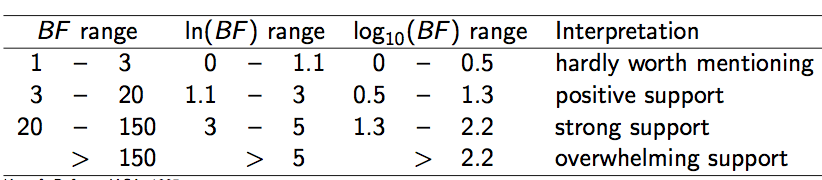
\includegraphics[width=0.800000\textwidth]{figures/BFs.png}
    \caption{Bayes factor support.}
\end{figure}

Note that sometimes a factor 2 is used for multiplying BFs, so when
comparing BFs from different publications, be aware which definition was
used.

\textbf{Nested sampling} is an algorithm that works as follows:

\begin{itemize}

\item
  randomly sample \lstinline!N! points from the prior
\item
  while not converged	

  \begin{itemize}
  
  \item
    pick the point with the lowest likelihood $L_{min}$, and save to log file
  \item
    replace the point with a new point randomly sampled from the prior
    using an MCMC chain of \lstinline!subChainLength! samples
    \textbf{under the condition that the likelihood is at least $L_{min}$}
  \end{itemize}
\end{itemize}

So, the main parameters of the algorithm are the number of particles
\lstinline!N! and the \lstinline!subChainLength!. \lstinline!N! can be
determined by starting with \lstinline!N=1! and from the information of
that run a target standard deviation can be determined, which gives us a
formula to determine \lstinline!N! (as we will see later in the
tutorial). The \lstinline!subChainLength! determines how independent the
replacement point is from the point that was saved, and is the only
parameter that needs to be determined by trial and error -- see
\protect\hyperlink{nested-sampling-faq}{FAQ} for details.

\clearpage

\section{Programs used in this
tutorial}\label{programs-used-in-this-tutorial}

\subsubsection{BEAST2 - Bayesian Evolutionary Analysis Sampling Trees
2}\label{beast2---bayesian-evolutionary-analysis-sampling-trees-2}

BEAST2 is a free software package for Bayesian evolutionary analysis of
molecular sequences using MCMC and strictly oriented toward inference
using rooted, time-measured phylogenetic trees \citep{Bouckaert2014},
\citep{bouckaert2018beast}. This tutorial uses the BEAST2 version 2.5.2.

\subsubsection{BEAUti2 - Bayesian Evolutionary Analysis
Utility}\label{beauti2---bayesian-evolutionary-analysis-utility}

BEAUti2 is a graphical user interface tool for generating BEAST2 XML
configuration files.

Both BEAST2 and BEAUti2 are Java programs, which means that the exact
same code runs on all platforms. For us it simply means that the
interface will be the same on all platforms. The screenshots used in
this tutorial are taken on a Mac OS X computer; however, both programs
will have the same layout and functionality on both Windows and Linux.
BEAUti2 is provided as a part of the BEAST2 package so you do not need
to install it separately.

\subsubsection{Tracer}\label{tracer}

\href{http://tree.bio.ed.ac.uk/software/tracer}{Tracer} is used to
summarise the posterior estimates of the various parameters sampled by
the Markov Chain. This program can be used for visual inspection and to
assess convergence. It helps to quickly view median estimates and 95\%
highest posterior density intervals of the parameters, and calculates
the effective sample sizes (ESS) of parameters. It can also be used to
investigate potential parameter correlations. We will be using Tracer
v1.7.0. \clearpage

\section{Practical: Selecting a clock
model}\label{practical-selecting-a-clock-model}

We will analyse a set of hepatitis B virus (HBV) sequences sampled
through time and concentrate on selecting a clock model. The most
popular clock models are the strict clock model and uncorrelated relaxed
clock with log normal distributed rates (UCLN) model.

\subsection{Setting up the Strict clock
analysis}\label{setting-up-the-strict-clock-analysis}

First thing to do is set up the two analyses in BEAUti, and run them in
order to make sure there are differences in the analyses. The alignment
can be downloaded here:
\url{https://raw.githubusercontent.com/rbouckaert/NS-tutorial/master/data/HBV.nex}.
We will set up a model with tip dates, HKY substitution model,
Coalescent prior with constant population, and a fixed clock rate.

\begin{framed}
\textbf{In BEAUti:}

\begin{itemize}

\item
  Start a new analysis using the Standard template.
\item
  Import
  \href{https://raw.githubusercontent.com/rbouckaert/NS-tutorial/master/data/HBV.nex}{HBV.nex}
  using menu \lstinline!File > Import alignment!.
\item
  In the tip-dates panel, select \lstinline!tip dates!, click
  \lstinline!Auto configure! and select the
  \lstinline!split on character! option, taking group 2 (see
  \protect\hyperlink{fig:auto-config}{Fig 2}).
\item
  In the site model panel, select \lstinline!HKY! as substitution model
  and leave the rest as is.
\item
  In the clock model panel, set the clock rate to 2e-5. Though usually,
  we want to estimate the rate, to speed things up for the tutorial, we
  fix the clock rate at that number as follows:

  \begin{itemize}
  
  \item
    Uncheck menu \lstinline!Mode > Automatic set clock rate!. Now the
    estimate entry should not be grayed out any more.
  \item
    Uncheck the \lstinline!estimate! box next to the clock rate entry.
  \end{itemize}
\item
  In the priors panel, select \lstinline!Coalescent Constant Population!
  as tree prior.
\item
  Also in the priors panel, change to \lstinline!popSize! prior to
  \lstinline!Gamma! with alpha = 0.01, beta = 100
  (\protect\hyperlink{fig:priors}{Fig 3}).
\item
  In the MCMC panel, change the \lstinline!Chain Length! to 1 million.
\item
  You can rename the file for trace log and tree file to include
  ``Strict'' to distinguish them for the relaxed clock ones.
\item
  Save the file as \lstinline!HBVStrict.xml!. \textbf{Do not close
  BEAUti just yet!}
\item
  Run the analysis with BEAST.
\end{itemize}
\end{framed}

\begin{framed}
\textbf{Do you have a clock rate prior in the priors panel?} If so, the
clock rate is estimated, and you should revisit the part where the clock
is set up!
\end{framed}

\begin{figure}
    \centering
    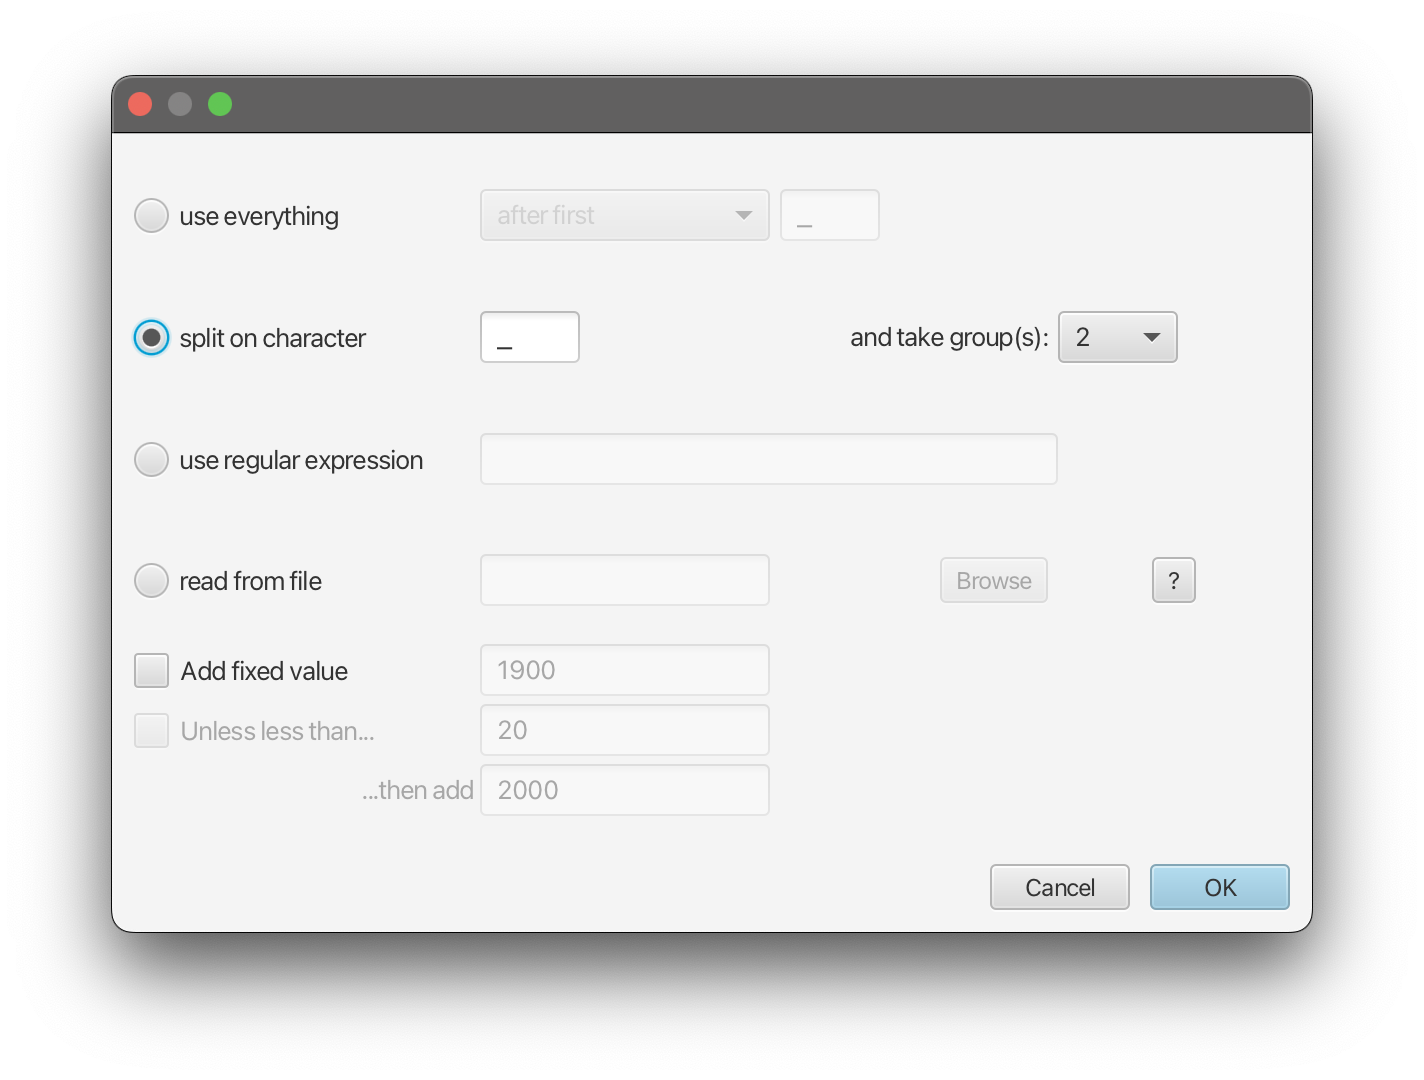
\includegraphics[width=0.800000\textwidth]{figures/BEAUti-configure-tip-dates.png}
    \caption{Configuring tip dates in BEAUti}
\end{figure}

\begin{figure}
    \centering
    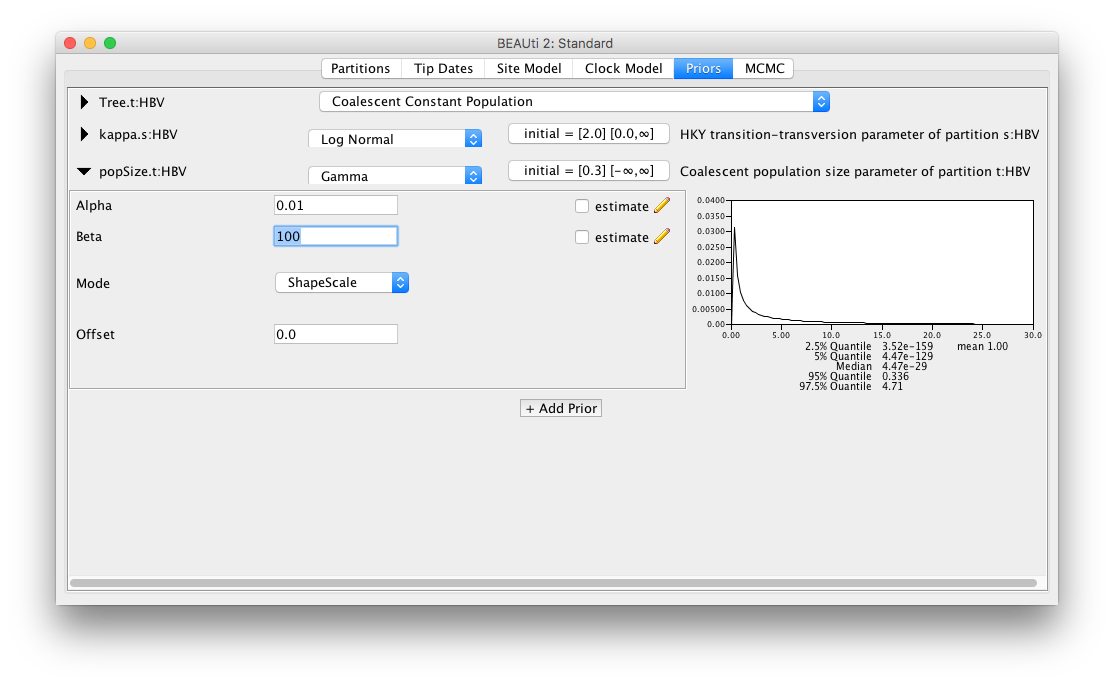
\includegraphics[width=0.800000\textwidth]{figures/BEAUti-priors.png}
    \caption{Priors panel for strict clock analysis in BEAUti}
\end{figure}

\subsection{Setting up the relaxed clock
analysis}\label{setting-up-the-relaxed-clock-analysis}

\begin{framed}
While you are waiting for BEAST to finish, it is time to set up the
relaxed clock analysis. This is now straightforward if BEAUti is still
open (if BEAUti was closed, open BEAUti, and load the file
\lstinline!HBVStrict.xml! through the menu \lstinline!File > Load!):

\begin{itemize}

\item
  In the clock model panel, change \lstinline!Strict clock! to
  \lstinline!Relaxed Clock Log Normal!.
\item
  Set the clock rate to 2e-5, and uncheck the \lstinline!estimate! box.
\item
  In the MCMC panel, replace \lstinline!Strict! in the file names for
  trace and tree log to \lstinline!UCLN!.
\item
  Save file as \lstinline!HBVUCLN.xml! \textbf{Do not click the
  \lstinline!File > Save! menu, but \lstinline!File > Save as!,
  otherwise the strict clock XML file will be overwritten}
\item
  Run the analysis in BEAST
\end{itemize}
\end{framed}

Once the analyses have run, open the log file in Tracer and compare
estimates and see whether the analyses substantially differ. You can
also compare the trees in DensiTree.

\begin{framed}
Are there any statistics that are very different? Do tree heights differ
substantially? Which analysis is preferable and why?
\end{framed}

If there are no substantial differences between the analysis for the
question you are interested in, you do not have to commit to one model
or another, and you can claim that the results are robust under
different models. However, if there are significant differences, you may
want to do a formal test to see which model is preferred over other
models. In a Bayesian context, in practice this comes down to estimating
the marginal likelihood, and calculating Bayes factors: the ratios of
marginal likelihoods. Nested sampling \citep{russel2018model} is one way
to estimate marginal likelihoods.

\subsection{Installing the NS Package}\label{installing-the-ns-package}

To use nested sampling, first have to install the NS (version \{\{
page.nsversion \}\} or above) package.

\begin{framed}
Open BEAUti and navigate to \textbf{File \textgreater{} Manage
Packages}. Select NS and then click \textbf{Install/Upgrade}
(\protect\hyperlink{fig:install}{Fig 4}). Then \textbf{\emph{restart
BEAUti}} to load the package.
\end{framed}

\begin{figure}
    \centering
    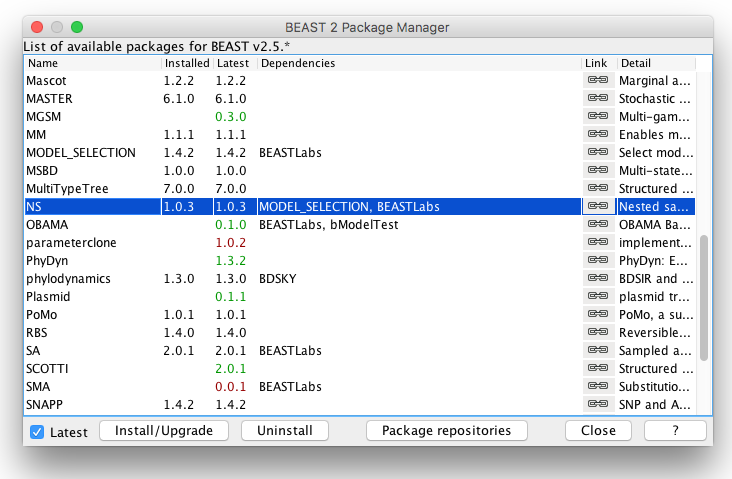
\includegraphics[width=0.800000\textwidth]{figures/install_NS.png}
    \caption{Installing NS in the Manage Packages window in BEAUti}
    \label{fig:install}
\end{figure}

\subsection{Setting up the nested sampling
analyses}\label{setting-up-the-nested-sampling-analyses}

\begin{framed}
\begin{itemize}

\item
  copy the file \lstinline!HBVStrict.xml! to \lstinline!HBVStric-NS.xml!
  and
\item
  copy \lstinline!HBVUCLN.xml! to \lstinline!HBVUCLN-NS.xml!
\item
  start a text editor and in both copied files, change
\end{itemize}

\begin{lstlisting}[language=XML]
<run id="mcmc" spec="MCMC" chainLength="1000000">
\end{lstlisting}

to

\begin{lstlisting}[language=XML]
<run id="mcmc" spec="beast.gss.NS" chainLength="20000" particleCount="1" subChainLength="5000">
\end{lstlisting}

\begin{itemize}

\item
  Here the \lstinline!particleCount! represents the number of active
  points used in nested sampling: the more points used, the more
  accurate the estimate, but the longer the analysis takes. The
  \lstinline!subChainLength! is the number of MCMC samples taken to get
  a new point that is independent (enough) from the point that is saved.
  Longer lengths mean longer runs, but also more independent samples. In
  practice, running with different \lstinline!subChainLength! is
  necessary to find out which length is most suitable (see
  \protect\hyperlink{nested-sampling-faq}{FAQ}).
\item
  change the file names for the trace and tree log to include
  \lstinline!NS! (searching for \lstinline!fileName=! will get you there
  fastest).
\item
  save the files, and run with BEAST.
\end{itemize}
\end{framed}

The end of the BEAST run for nested sampling with the strict clock
should look something like this:

\begin{lstlisting}
Total calculation time: 34.146 seconds
End likelihood: -202.93224422946253
Producing posterior samples

Marginal likelihood: -12438.35758179847 sqrt(H/N)=(11.084732655710818)=?=SD=(11.008249475863373) Information: 122.87129804858182
Max ESS: 6.706301939836118


Processing 248 trees from file.
Log file written to HBVStrict-NS.posterior.trees
Done!

Marginal likelihood: -12437.767705819117 sqrt(H/N)=(11.05930077842042)=?=SD=(11.71074051847201) Information: 122.3081337075705
Max ESS: 6.490414156277384


Log file written to HBVStrict-NS.posterior.log
Done!
\end{lstlisting}

and for the relaxed clock:

\begin{lstlisting}
Total calculation time: 38.541 seconds
End likelihood: -200.7794173971489
Producing posterior samples

Marginal likelihood: -12428.557546706481 sqrt(H/N)=(11.22272275528845)=?=SD=(11.252847709777592) Information: 125.94950604206919
Max ESS: 5.874085822198268


Processing 257 trees from file.
Log file written to HBVUCLN-NS.posterior.trees
Done!

Marginal likelihood: -12428.480923049345 sqrt(H/N)=(11.220392192278625)=?=SD=(11.491864352217954) Information: 125.89720094854714
Max ESS: 5.940996269769591


Log file written to HBVUCLN-NS.posterior.log
Done!
\end{lstlisting}

As you can see, nested sampling produces estimates of the marginal
likelihood as well as standard deviation estimates. At first sight, the
relaxed clock has a log marginal likelihood estimate of about -12428,
while the strict clock is much worse at about -12438. However, the
standard deviation of both runs is about 11, so that makes these
estimates indistinguishable. Since this is a stochastic process, the
exact numbers for your run will differ, but should not be that far
appart (less than 2 SDs, or about 22 log points in 95\% of the time).

To get more accurate estimates, the number of particles can be
increased. The expected SD is sqrt(H/N) where N is the number of
particles and H the information. The information H is conveniently
estimated in the nested sampling run as well. To aim for an SD of say 2,
we need to run again with N particles such that 2=sqrt(125/N), which
means 4=125/N, so N=125/4 and N=32 will do. Note that the computation
time of nested sampling is linear in the number of particles, so it will
take about 32 times longer to run if we change the particleCount from 1
to 32 in the XML.

A pre-cooked run with 32 particles can be found here:
\url{https://github.com/rbouckaert/NS-tutorial/tree/master/precooked_runs}.
Download the files
\href{https://raw.githubusercontent.com/rbouckaert/NS-tutorial/master/precooked_runs/HBVStrict-NS32.log}{HBV-Strict-NS32.log}
and
\href{https://raw.githubusercontent.com/rbouckaert/NS-tutorial/master/precooked_runs/HBVUCLN-NS32.log}{HBVUCLN-NS32.log}
and run the \lstinline!NSLogAnalyser! application to analyse the
results. To start the \lstinline!NSLogAnalyser! from the command line,
use

\begin{lstlisting}
applauncher NSLogAnalyser -noposterior -N 32 -log /path/to/HBVStrict-NS32.log
applauncher NSLogAnalyser -noposterior -N 32 -log /path/to/HBVUCLN-NS32.log
\end{lstlisting}

or from BEAUti, click menu \lstinline!File/Launch apps!, select
\lstinline!NSLogAnalyser! and fill in the form in the GUI. The output
for the strict clock analysis should be something like this:

\begin{lstlisting}
Loading HBVStrict-NS32.log, burnin 0%, skipping 0 log lines

|---------|---------|---------|---------|---------|---------|---------|---------|
******************************

Marginal likelihood: -12426.207750474812 sqrt(H/N)=(1.8913059067381148)=?=SD=(1.8374367294317693) Information: 114.46521705159945
Max ESS: 400.41214209052896

Calculating statistics

|---------|---------|---------|---------|---------|---------|---------|---------|
********************************************************************************

#Particles = 32
item               mean     stddev   
posterior          -12512.7 2.988107
likelihood         -12311.7 2.91633 
prior              -201.009 1.580207
treeLikelihood     -12311.7 2.91633 
TreeHeight         3443.955 134.1921
kappa              2.679169 0.151243
popSize            2337.454 290.0407
CoalescentConstant -163.191 3.090671
freqParameter.1    0.240033 0.005884
freqParameter.2    0.267856 0.006814
freqParameter.3    0.217084 0.006638
freqParameter.4    0.275027 0.006716
Done!
\end{lstlisting}

So, that gives us a ML estimate of -12426.2 with SD of 1.89, slightly
better than the 2 we aimed for, but the information is also a bit lower
than we assumed (114 vs 128). Furthermore, there are posterior estimates
of all the entries in the trace log. Nested sampling does not only
estimate MLs and SDs, but can also provide a sample from the posterior,
which can be useful for cases where MCMC has trouble with convergence.
But let's not digress too much and get back to model selection.

For the relaxed clock analysis, we get something like:

\begin{lstlisting}
Marginal likelihood: -12417.389793288146 sqrt(H/N)=(1.9543337689486355)=?=SD=(1.9614418034828585) Information: 122.2214553744953
\end{lstlisting}

so an ML of -12417.4 with SD of 1.95. Therefor the log BF is -12417.4 -
-12426.2 = 8.8, which is more than twice the sum of the SDs, so can be
considered reliable evidence in favour of the relaxed clock model. Note
that judging from the table at the start of the tutorial, this amounts
to overwhelming support for the relaxed clock.

\hypertarget{nested-sampling-faq}{\section{Nested sampling
FAQ}\label{nested-sampling-faq}}

\subsection{The analysis prints out multiple ML estimates with their
SDs. Which one to
choose?}\label{the-analysis-prints-out-multiple-ml-estimates-with-their-sds.-which-one-to-choose}

The difference between the estimates is the way they are estimated from
the nested sampling run. Since these are estimates that require random
sampling, they differ from one estimate to another. When the standard
deviation is small, the estimates will be very close, but when the
standard deviations is quite large, the ML estimates can substantially
differ. Regardless, any of the reported estimates are valid estimates,
but make sure to report them with their standard deviation.

\subsection{How do I know the sub-chain length is large
enough?}\label{how-do-i-know-the-sub-chain-length-is-large-enough}

NS works in theory if and only if the points generated at each iteration
are independent. If you already did an MCMC run and know the effective
sample size (ESS) for each parameter, to be sure every parameter in
every sample is independent you can take the length of the MCMC run
divided by the smallest ESS as sub-chain length. This tend to result in
quite large sub-chain lengths.

In practice, we can get away much smaller sub-chain lengths, which you
can verify by running multiple NS analysis with increasing sub-chain
lengths. If the ML and SD estimates do not substantially differ, you
know the shorter sub-chain length was sufficient.

\subsection{How many particles do I
need?}\label{how-many-particles-do-i-need}

To start, use only a few particles. This should give you a sense of the
information \lstinline!H!, which is one of the estimates provided by the
NS analysis. If you want to compare two hypotheses, you want the
difference between \lstinline!ML1! and \lstinline!ML2! to be at least
\lstinline!2*sqrt(SD1*SD1+SD2*SD2)! in order to make sure the difference
is not due to randomisation.

If the difference is larger, you do not need more particles.

If the difference is smaller, you can guess how much the SD estimates
must shrink to get a difference that is sufficiently large. Since the
\lstinline!SD=sqrt(H/N)!, we have that \lstinline!N=H/(SD*SD)! and
\lstinline!H! comes from the NS run with a few particles. Run the
analysis again, with the increased number of particles, and see if the
difference becomes large enough.

If the difference is less than 2, the hypotheses may not be
distinguishable -- in terms of Bayes factors, are barely worth
mentioning.

\subsection{Is NS faster than path sampling/stepping stone
(PS/SS)?}\label{is-ns-faster-than-path-samplingstepping-stone-psss}

This depends on many things, but in general, depends on how accurate the
estimates should be. For NS, we get an estimate of the SD, which is not
available for PS/SS. If the hypotheses have very large differences in
MLs, NS requires very few (maybe just 1) particle, and will be very
fast. If differences are smaller, more particles may be required, and
the run-time of NS is linear in the number of particles.

The parallel implementation makes it possible to run many particles in
parallel, giving a many-particle estimate in the same time as a single
particle estimate (PS/SS can be parallelised by steps as well).

\subsection{The output is written on screen, which I forgot to save. Can
I estimate them directly from the log
files?}\label{the-output-is-written-on-screen-which-i-forgot-to-save.-can-i-estimate-them-directly-from-the-log-files}

The NS package has a \lstinline!NSLogAnalyser! application that you can
run via the menu \lstinline!File/Launch apps! in BEAUti -- a window pops
up where you select the \lstinline!NSLogAnalyser!, and a dialog shows
you various options to fill in. You can also run it from the command
line on OS X or Linux using

\begin{lstlisting}
/path/to/beast/bin/applauncher NSLogAnalyser -N 1 -log  xyz.log
\end{lstlisting}

where the argument after \lstinline!N! is the \lstinline!particleCount!
you specified in the XML, and \lstinline!xyz.log! the trace log produced
by the NS run.

\subsection{Why are some NS runs longer than
others?}\label{why-are-some-ns-runs-longer-than-others}

Nested sampling stops automatically when the accuracy in the ML estimate
cannot be improved upon. Because it is a stochastic process, some
analyses get there faster than others, resulting in different run times.

\subsection{Why are the ESSs so low when I open a log file in
Tracer?}\label{why-are-the-esss-so-low-when-i-open-a-log-file-in-tracer}

An NS analysis produces two trace log files: one for the nested sampling
run (say \lstinline!myFile.log!) and one with the posterior sample
(\lstinline!myFile.posterior.log!).

The ESSs in Tracer of log files with the posterior samples are
meaningless, because the log file is ordered using the nested sampling
run. If you look at the trace of the Likelihood, it should show a
continuous increasing function. It is not quite clear how to estimate
ESSs of a nested sampling run yet, though the number of entries in the
posterior log is equal to the maximum theoretical ESS, which is almost
surely an overestimate.

\clearpage

\section{Useful Links}\label{useful-links}

\begin{itemize}

\item
  \href{http://www.beast2.org/book.html}{Bayesian Evolutionary Analysis
  with BEAST 2} \citep{BEAST2book2014}
\item
  BEAST 2 website and documentation: \url{http://www.beast2.org/}
\item
  Nested sampling website and documentation:
  \url{https://github.com/BEAST2-Dev/nested-sampling}
\item
  Join the BEAST user discussion:
  \url{http://groups.google.com/group/beast-users}
\end{itemize}



%%%%%%%%%%%%%%%%%%%%%%%
% Tutorial disclaimer %
%%%%%%%%%%%%%%%%%%%%%%%
% Please do not change the license
% Add the author names and relevant links
% Add any other aknowledgments here
\href{http://creativecommons.org/licenses/by/4.0/}{
\includegraphics[scale=0.8]{figures/ccby.pdf}} This tutorial was written by Remco Bouckaert for \href{https://taming-the-beast.github.io}{Taming the BEAST} and is licensed under a \href{http://creativecommons.org/licenses/by/4.0/}{Creative Commons Attribution 4.0 International License}. 


%%%%%%%%%%%%%%%%%%%%
% Do NOT edit this %
%%%%%%%%%%%%%%%%%%%%
Version dated: \today



%\newpage

%%%%%%%%%%%%%%%%
%  REFERENCES  %
%%%%%%%%%%%%%%%%

\printbibliography[heading=relevref]


\end{document}